


\documentclass{Beamer}

% To make a numbered table of contents as in chapters of
% a book
\setbeamertemplate{section in toc}[sections numbered]
\setbeamertemplate{subsection in toc}[subsections numbered]

%In beamer presentation, the packages must be included in the same file, it doesn't work as in 


%*********** Input Macros and Packages ******************

\input{Files/Macros}

% for design
%\usetheme{Warsaw}

% Add support for \subsubsectionpage
\def\subsubsectionname{\translate{Subsubsection}}
\def\insertsubsubsectionnumber{\arabic{subsubsection}}

\setbeamertemplate{subsubsection page}
{
  \begin{centering}
    {\usebeamerfont{subsubsection name}\usebeamercolor[fg]{subsubsection name}}
    \vskip1em\par
    \begin{beamercolorbox}[sep=4pt,center]{part title}
      \usebeamerfont{subsubsection title}\insertsubsubsection\par
    \end{beamercolorbox}
  \end{centering}
}

%https://tex.stackexchange.com/questions/117658/automatically-generate-section-title-slides-in-beamer/117661

\def\subsubsectionpage{\usebeamertemplate*{subsubsection page}}

%\AtBeginSection{\frame{\sectionpage}}
%\AtBeginSubsection{\frame{\subsectionpage}}

% Automatically define something at the begnining
% of each subsubsection
\AtBeginSubsubsection{\frame{\subsubsectionpage}}

\useoutertheme{infolines}

\usecolortheme{seahorse}

% Slide Number: display slide number/ total number of slides

\setbeamertemplate{footline}[frame number]


% References and Biblio
\setbeamertemplate{bibliography item}{\insertbiblabel}

\setbeamertemplate{navigation symbols}{}



% Foot Options: deafult controls off
\usenavigationsymbolstemplate{} 

% Fonts:changes fonts, make the equation writing more
% fancy
\usefonttheme{professionalfonts} 


\usepackage{xcolor}

\usepackage{graphicx,caption}


% Math Opeartor
\DeclareMathOperator*{\argmax}{argmax}


\usepackage{multicol}



%************ End of Packages *****************

%*****************************************
%*****************************************
%*****************************************

\title[Acronym]{Digital Communication}
%\subtitle{Subtitle Here}
\author{Ranim Tom}
%\institute{Supervisors: Supervisors Names}

%In case I don't want the date to appear in the slides
\date[]

\begin{document}

%\metroset{block=fill}

\begin{frame}
\titlepage
\end{frame}

% Displaying Table of Contents
\begin{frame}[t,allowframebreaks]{Table of Contents}
\tableofcontents
%This command if we want to display only sections
%without subsections
%\tableofcontents[hideallsubsections]
\end{frame}


%*********** Start Creating Slides **************



\section{Preface}
\label{Chap:Preface}
\begin{frame}[t]{Chapter \autoref{Chap:Preface}}
\tableofcontents[sections= \value{section}]
\end{frame}

\begin{frame}[t]{Preface}


\end{frame}


\section{Baseband Binary Communication}
\label{Chap:Baseband_Binary_Communication}
\begin{frame}[t]{Chapter \autoref{Chap:Baseband_Binary_Communication}}
\tableofcontents[sections= \value{section}]
\end{frame}



\subsection{Introduction}
\begin{frame}[t]{Introduction}

\begin{itemize}

\item In this chapter, we deal only with \textcolor{red}{baseband communication:}

	\begin{itemize}
	\item \textcolor{red}{Amplitude Spectrum} of the signal is \textcolor{red}{centered at 0 Hz}
	
	\item No carrier signal is used for transmission $\leftrightarrow$ no modulation
	
	\end{itemize}

\item Modulation Scheme will be addressed in later chapters

\item Many of the important concept done in this chapter are generalized in modulation scheme also (this chapter isn't a waste of time)

	\begin{itemize}
	\item Detection
	
	\item Bits assignments
	
	\item $\cdots$
	\end{itemize}

\end{itemize}


\end{frame}


\subsubsection{Transmitting Binary Data}
\begin{frame}[t,allowframebreaks]{Transmitting Binary Data}

\begin{itemize}

\item One important thing to note in \textcolor{red}{digital communication} is that the \textcolor{red}{message} we transmit is a \textcolor{red}{stream of bits}: 0 and 1

\item This has the advantage to let the \textcolor{red}{receiver} to \textcolor{red}{decide between 2 values} only when doing detection

	\begin{itemize}
	\item In opposite to analog communication, where the received signal has infinite amount of values
	
	\item So if we have noise, it is hard to do detection
	\end{itemize}


\end{itemize}

\end{frame}


\begin{frame}[t]{Binary Communication System}

\begin{itemize}

\item We begin first by \textcolor{red}{binary communication system}

	\begin{itemize}
	
	\item We have only \textcolor{red}{1 bit to transmit}: 0 or 1	
	
	\item We have \textcolor{red}{2 signals}: $s_1(t)$ for bit 0 and $s_2(t)$ for bit 1
	\end{itemize}

\item These bits comes from the analog to digital process (digital signal processing classes)

	\begin{itemize}
	\item In this class, we directly assume that these steps are done correctly and we have directly the stream of bits which we want to transmit
	\end{itemize}

\end{itemize}


\end{frame}

\subsubsection{General Communication System and Mapping}
\begin{frame}[t,allowframebreaks]{General Communication System and Mapping}

\begin{itemize}

\item In general, we could also transmit more than 1 bit:

	\begin{itemize}
	\item For example if we have 2 bits, we have $2^2$ possible combination: 00, 01, 10 and 11
	
	\item Thus we will have 4 signals $s_M(t)$ where $M \, = \, 2^n \, = \, $ \textcolor{red}{number of symbols (signals)} to be transmitted
	\end{itemize}

\item Usually in every digital communication system, we have to do a \textcolor{red}{mapping} of the stream bits to a set of signals 

	\begin{itemize}
	\item $N$ bits $b_0 \, , \, b_1 \, , \, b_2 \, \cdots \, b_{N \, - \, 1} \mapsto \, \text{a set of  } M \, \text{ signals } {\, s_i(t): 0 \, \leq \, i \, \leq M \, - \, 1 \, }$ 
	\end{itemize}

\item In case we have \textcolor{red}{more than 1 bit to transmit} $\leftrightarrow$ \textcolor{red}{more than 2 transmitted signal}, the communication system is referred to as \textcolor{red}{M-ary communication}

\newpage
\item In \textcolor{red}{this chapter} we deal with the \textcolor{red}{special case of an M-ary communication} $\leftrightarrow$ binary communication system:

	\begin{itemize}
	\item $M \, = \, 2 \rightarrow$ 2 signals $s_0(t)$ and $s_1(t)$, and we have 1 bit in each signal: 0 or 1
	\end{itemize}	 

\end{itemize}


\end{frame}


\subsubsection{Digital Waveform}
\begin{frame}[t]{Digital Waveform}

\begin{itemize}

\item The signals $s_i(t)$ are assumed to be \textcolor{red}{time limited} with a symbol duration denoted by $T_{\text{symbol}}$

\item In binary communication system, in the period $T_{\text{symbol}}$ we transmit only 0 or 1

\end{itemize}

\begin{figure}[h]
\centering
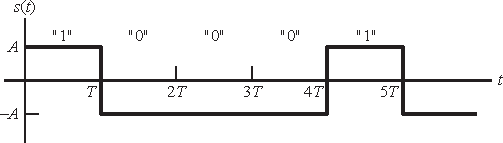
\includegraphics[scale=0.8]{Figures/Baseband_Binary/template_digital_signal}
\caption{$T$ here is $T_{\text{symbol}}$}
\label{fig:Baseband_Binary:template_digital_signal}
\end{figure}

\begin{itemize}

\item For transmission, the \textcolor{red}{bits} (0 and 1) are \textcolor{red}{mapped} to {electrical signals} using what we call \textcolor{red}{line coding techniques}

\end{itemize}



\end{frame}


\subsubsection{Synchronization}
\begin{frame}[t,allowframebreaks]{Synchronization and Receiver Knowledge}

\begin{itemize}

\item Throughout this chapter, we assume that the Rx knows where each pulse start and finish

\end{itemize}


\end{frame}



\subsubsection{Orthogonality Reminder}
\begin{frame}[t,allowframebreaks]{Orthogonality Reminder}

\begin{itemize}

\item 2 signals are orthogonal on $[0,t]$ if their inner product is 0

\begin{equation}
\displaystyle\int\limits_0^t x(t) \, y(t) \, dt \, = \, 0
\end{equation}

	\begin{itemize}
	\item This means that if we project $x(t)$ onto $y(t)$, $x(t)$ has no component on $y(t)$
	\end{itemize}

\item For a set of $M$ signals as in the case of $M$-ary communication, we must verify the equality between all paired signals

\begin{equation}
\displaystyle\int\limits_0^{T_{\text{symbol}}} s_i(t) \, s_j(t) \, dt \, = \, 0 \quad \forall \, i,j \text{ with } i \, \neq \, j
\end{equation}

\end{itemize}


\end{frame}



\subsection{Linear Receiver}

\begin{frame}[t]{Introduction}

\begin{itemize}

\item Usually when explaining some concept, there are 2 ways to proceeds:

	\begin{enumerate}
	\item Do directly a \textcolor{red}{general derivation}
	
	\item The opposite case: take \textcolor{red}{a specific example}, and then \textcolor{blue}{generalize this example}
	\end{enumerate}

\item In the following slides, we adopt approach 2 for \textcolor{red}{receiver} study for a \textcolor{red}{base band binary communication system} 

\end{itemize}

\end{frame}

\begin{frame}[t,allowframebreaks]{A Proposed Model for the Receiver}

\begin{itemize}

\item The received signal is the sum of the transmitted signals plus the noise component which model the channel corruption

\begin{equation}
y_{\text{R}_x}(t) \, = \, s_i(t) \, + \, n(t)
\end{equation}

	\begin{itemize}
	\item $s_i(t)$ is either $s_1(t)$ or $s_2(t)$ since we are in digital binary communication system
	\end{itemize}


\begin{figure}[h]
\centering
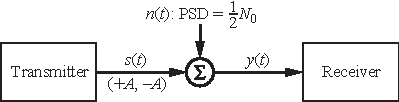
\includegraphics[scale=0.8]{Figures/Baseband_Binary/block_rx_signa_and_noise}
\label{fig:Baseband_Binary:block_rx_signa_and_noise}
\end{figure}


\item Mathematical Assumption:

	\begin{itemize}
	\item White Gaussian Noise with PSD $\displaystyle\frac{N_0}{2}$
	
	\item The signals are:$ \begin{cases}
	s_1(t) \, = \, - \, \text{Amp} \, \times \,  p_T(t) \quad \text{for bit 0} \\
	s_2(t) \, = \, + \, \text{Amp} \,  \times \,  p_T(t) \quad \text{for bit 1}
	\end{cases}$
	

	\end{itemize}


\item We will consider \textcolor{red}{a} receiver model shown in figure \autoref{fig:Baseband_Binary:integrate_rx_binary}.

\begin{figure}[h]
\centering
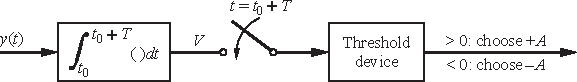
\includegraphics[scale=0.8]{Figures/Baseband_Binary/integrate_rx_binary}
\caption{Integrate-and-dump Rx}
\label{fig:Baseband_Binary:integrate_rx_binary}
\end{figure}
		
\item \underline{\textit{Receiver Steps}} : Several \textcolor{red}{Steps} of processing will be done to the received signal $y_{R_x}(t)$

	\begin{enumerate}
	\item \textcolor{red}{Integration} over the symbol duration:
	
		\begin{itemize}
		\item The output of the integrator will be some number
		
		\item The integration done here is some kind of \textcolor{red}{filtering} 
		\end{itemize}
		
		\item \textcolor{red}{Compare} the output of the integration to 	some \textcolor{red}{threshold}
	\end{enumerate}

\end{itemize}


\end{frame}





\subsubsection{Integration Output}

\begin{frame}[t]{Probabilistic Integration}

\begin{itemize}

\item The \textcolor{red}{integration step} involves a \textcolor{red}{probabilistic quantity} since the received signal $y_{R_x}(t)$ is random due to the noise component $n(t)$

\item What we will do in this part is the \textcolor{red}{computation of this integration} to understand how the linear receiver of  figure work

\item Notation: We will denote the \textcolor{red}{output of the integration} by $V$

	\begin{itemize}
	\item $V$ is a \textcolor{red}{decision statistics} which depends on the transmitted signal $s_i(t)$
	\end{itemize}

\item To do the computation for $V$ and derive its distribution, we do the following assumption that $s_2(t)$ is transmitted (positive pulse +Amp)

	\begin{itemize}
	\item Hence $V$ is know will be denoted by $V_2$ where the \textcolor{red}{subscript} denote the distribution of $V$ \textcolor{red}{given that $s_2(t)$ is transmitted} $\leftrightarrow$ it is a \textcolor{red}{conditional distribution}
	
	\item Same concept for $V_1 \, \leftrightarrow \, s_1(t)$ (\textcolor{red}{negative pulse -Amp}) is transmitted conditional distribution given that 
	\end{itemize}

\end{itemize}

\end{frame}

\begin{frame}[t,allowframebreaks]{Computation Steps for Probabilistic Integration of Positive Pulse}

\begin{enumerate}

\item General Formula at the output of the receiver:

\begin{equation}
V \, = \, \displaystyle\int\limits_{0}^{T_{\text{symbol}}} s_i(t) \, + \, n(t)
\end{equation}

\item Assume that $s_1(t)$ is transmitted hence $s_i(t) \, = \, s_2(t)$ and $Z\, \rightarrow \, V_2$

\begin{equation}
V_2 \, = \, \displaystyle\int\limits_{0}^{T_{\text{symbol}}} s_2(t) \, + \, n(t)
\end{equation}

\item Decompose the integral:

\begin{equation}
V_2 \, = \, \underbrace{\displaystyle\int\limits_{0}^{T_{\text{symbol}}} s_1(t)}_{\text{Determnisitic}}  \, + \,   \underbrace{\displaystyle\int\limits_{0}^{T_{\text{symbol}}}n(t)}_{\text{Random}}
\end{equation}

	\begin{itemize}
	\item $s_2(t)$ is a rectangular pulse with a width of $ T_{symbol}$ and height equal to a certain amplitude $\rightarrow$ the integral is equal to $ \text{Amp}\, \times \, T_{symbol}$
	
	\item $n(t)$ is a Gaussian process, but the integral of a Gaussian is a Gaussian and if we sum a Gaussian random variable to a deterministic quantity, we obtain a Gaussian random variable also $\rightarrow \, Z_2$ is a Gaussian random variable $\leftrightarrow$ we need its mean and variance to describe its conditional distribution
	\end{itemize}


\item  Hence we can write:

\begin{equation}
V_2 \, = \,  \text{Amp}\, \times \, T_{\text{symbol}} \, + \,   \displaystyle\int\limits_{0}^{T_{\text{symbol}}}n(t)  \, dt
\end{equation}

Since $Z_2$ is Gaussian, we now need to compute its mean $E[Z_2]$ and its variance $\text{Var}(Z_2)$.\\

Some Rules regarding mean computation:


	\begin{itemize}
	\item  Mean of a constant is a constant $ \leftrightarrow \, E[\text{constant}] \, = \, \text{constant}$
	
	\item Mean of a sum is the sum of the means $ \leftrightarrow \,  \,E[\, X \, + \, Y \, ] \, = \, E[X] \, + \, E[Y]$
	\end{itemize}




\newpage
\item Mean Computation:

$$\begin{array}{rcl}
E[V_2] \, &=& \, E \left[\, \text{Amp}\, \times \, T_{\text{symbol}} \, + \,   \displaystyle\int\limits_{0}^{T_{\text{symbol}}}n(t) \, dt   \,\right] \\ \\
		&=& \, E \left[\, \text{Amp}\, \times \, T_{\text{symbol}} \,\right]  \, + \, \underbrace{E \left[\, \displaystyle\int\limits_{0}^{T_{\text{symbol}}}n(t)  \, dt \,\right]}_{\text{Exchange the integrale and the E operator}}   \\ \\
		&=& \, \text{Amp}\, \times \, T_{\text{symbol}} \, + \, \,  \displaystyle\int\limits_{0}^{T_{\text{symbol}}}   E \left[\, n(t)  \,\right]  \, dt 
\end{array}$$

Since we are dealing with zero mean Gaussian process $\rightarrow \, E \left[\, n(t)  \,\right] \, = \, 0 \rightarrow \, \displaystyle\int\limits_{0}^{T_{\text{symbol}}}   E \left[\, n(t)  \,\right]  \, dt \, = \, \displaystyle\int\limits_{0}^{T_{\text{symbol}}} 0 \,  dt \, = \, 0$

and hence we have:

\begin{equation}
E[V_2] \, = \,  \text{Amp}\, \times \, T_{\text{symbol}}
\end{equation}


\newpage

\item Variance Computation:

\begin{itemize}
\item Recall the variance rule: $\text{Var}(X) \, = \, E \left[\,  \left(\, X \, - \, E[X]\, \right)^2  \,\right]$
\end{itemize}

$$\begin{array}{rcl}
\text{Var}(V_2) \, &=& \, E \left[\,  \left(\, V_2 \, - \, E[V_2]\, \right)^2  \,\right]
\label{Eq:baseband_com:variance_1}
\end{array}$$

where 

\begin{itemize}
\item $V_2 \, = \,  \text{Amp}\, \times \, T_{\text{symbol}} \, + \,   \displaystyle\int\limits_{0}^{T_{\text{symbol}}}n(t)  \, dt $

\item $E[V_2] \, = \,  \text{Amp}\, \times \, T_{\text{symbol}}$ 
\end{itemize}

Plugin those equations into equation (\autoref{Eq:baseband_com:variance_1}) we get:
 
\newpage

$\begin{array}{rcl}
\text{Var}(V_2) \,&=& \, E \left[\,  \left(\, \text{Amp}\, \times \, T_{\text{sym}} \, + \,   \displaystyle\int\limits_{0}^{T_{\text{sym}}}n(t)  \, dt \,  - \, \text{Amp}\, \times \, T_{\text{sym}} \, \right)^2  \,\right] \\ \\
&=& \, E \left[\, \left(\, \displaystyle\int\limits_{0}^{T_{\text{sym}}}n(t)  \, dt \, \right)^2  \,\right] \quad \text{decompose the integral} \\ \\
&=& \, E \left[\,  \displaystyle\int\limits_{0}^{T_{\text{sym}}}n(t)  \, dt \,  \times \, \displaystyle\int\limits_{0}^{T_{\text{sym}}}n(s)  \, ds   \,\right]\\ && \text{Exchange the E[.] and } \int 
\label{Eq:baseband_com:variance_2}
\end{array}$

\newpage
$\begin{array}{rcl}
\text{Var}(V_2) \,&=& \, \displaystyle\int\limits_{0}^{T_{\text{sym}}} \, \displaystyle\int\limits_{0}^{T_{\text{sym}}} \,  E \left[\,  n(t)  \, \times \, n(s)   \,\right] \, dt \, ds  
\end{array}$

\begin{itemize}
\item  $E \left[\,  n(t)  \, \times \, n(s)   \,\right]$ is the autorcorroleation at $(t,s)$ and its equal to $\displaystyle\frac{N_0}{2} \, \delta(\, t \, - \, s \,)$. 
\end{itemize}



$\begin{array}{rcl}
\text{Var}(V_2) \,&=& \, \displaystyle\frac{N_0}{2} \, \times \,  \displaystyle\int\limits_{0}^{T_{\text{sym}}} \, \displaystyle\int\limits_{0}^{T_{\text{sym}}} \, \delta(\, t \, - \, s \,) \, dt \, ds \\ \\
\end{array}$

	\begin{itemize}
	\item Let's think about the inner integral $\displaystyle\int\limits_{0}^{T_{\text{sym}}} \, \delta(\, t \, - \, s \,) \, dt$: here the $\delta(.)$ is a function of $t$, and it is located at $t \, = \, s$, and its area value (hence its  integral) equal to 1. Hence we have:
	\end{itemize}


$\begin{array}{rcl}
\text{Var}(V_2) \,&=& \, \displaystyle\frac{N_0}{2} \, \times \,  \displaystyle\int\limits_{0}^{T_{\text{sym}}} \, 1 \, dt \\ \\
&=& \, \displaystyle\frac{N_0 \, T_{\text{sym}}}{2}
\end{array}$

\newpage
\underline{Note:} need to review the integral trick we did in the double integration when we talk about the inner integral: why did we \textcolor{red}{drop} down $ds$ and let $dt$. This is done from random processes class when we deal with double integration for a $\delta(.)$ function.

\end{enumerate}

\end{frame}

\begin{frame}[t]{Summary of Computation}

\begin{itemize}

\item $E[V_2] \, = \,  \text{Amp}\, \times \, T_{\text{symbol}} \, \leftrightarrow$ location of the distribution $Z_2$

	\begin{itemize}
	\item So when I have symbol $s_1(t)$ transmitted, on average, I land on $  \text{Amp}\, \times \, T_{\text{symbol}}$
\end{itemize}	 

\item  $ \text{Var}(V_2) \, = \, \sigma^2 \, = \, \displaystyle\frac{N_0 \, T_{\text{sym}}}{2} \leftrightarrow$ the spread of the distribution $Z_2$

\item Same computation can be made for the conditional distribution $Z_1$: case where have as a given signal $s_1(t)$ (negative pulse -Amp) is transmitted

\end{itemize}


\end{frame}

\begin{frame}[t]{Distribution Plot}

\begin{figure}[h]
\centering
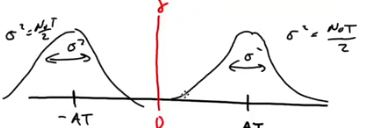
\includegraphics[scale=0.6]{Figures/Baseband_Binary/output_rx_distirbution}
\caption{Conditional Distribution Output of the Linear Receiver}
\label{fig:Baseband_Binary:output_rx_distirbution}
\end{figure}

\begin{itemize}

\item Regarding the threshold $k$, we have chosen $k \, = \, 0$

\item The reason to choose this and its effect will be discussed later

	\begin{itemize}
	\item How we can choose \textcolor{red}{optimum threshold value}
	\end{itemize}

\end{itemize}

\end{frame}



\begin{frame}[t,allowframebreaks]{Some Observation}

\begin{itemize}

\item The \textcolor{red}{variance} for \textcolor{red}{both signals} $s_1(t)$ and $s_2(t)$ is the \textcolor{red}{same}

	\begin{itemize}
	\item This indicates that the \textcolor{red}{channel corrupt the signal in the same way}, independently of the signals we transmit
	
	\item Notice also that the \textcolor{red}{variance} $\sigma^2$ \textcolor{red}{doesn't depends on the signals} $\rightarrow$ there is no index $i$ $\leftrightarrow$ it depends only on the noise $(N_0)$ and the duration $T_{\text{symbol}}$
	\end{itemize}

\item Regarding the mean which control the position of the curves:

	\begin{itemize}
	\item The amplitude controls the energy of the signals
	
	\item The higher the energy in our signals and if the noise still the same $\rightarrow$ the curves should be pushed further $\rightarrow$ the probability of error will decrease allot
	\end{itemize}
	
And this is very logical: the more energy we have $\rightarrow$ the more error decrease

\newpage
\item Always pay attention that our probability distribution should make sense

	\begin{itemize}
	\item We can't obtain for example the opposite result: the more energy we have, the more error we get $\leftrightarrow$ area of error will get bigger since the curves will get closer. That doesn't make sense.
	\end{itemize}

\end{itemize}

\end{frame}


\subsubsection{Performance Measure and Probability of Error}

\begin{frame}[t]{Performance Measure and Probability of Error}

\begin{itemize}

\item How we can know if the \textcolor{red}{Rx is good }or not for such a task?

\item A \textcolor{red}{performance measure} can be take is the \textcolor{red}{probability of error}. In this section we will compute it

\item In \textcolor{red}{binary digital communication}, the \textcolor{red}{error} can occur in \textcolor{red}{2 ways}:

\begin{enumerate}

\item  $s_1(t)$ is transmitted but the Rx detect $s_2(t)$ $\rightarrow \, P \, (\text{Error} \, | \, s_1(t) \text{ is sent})$ 

\item $s_2(t)$ is transmitted but the Rx detect $s_1(t)$ $\rightarrow \, P \, (\text{Error} \, | \, s_2(t) \text{ is sent})$ 

\end{enumerate}

\item Since the error can occur in 2 ways, so what we need to compute is the \textcolor{red}{total probability of error}

	\begin{itemize}
	\item This will be done using total probability rule
	\end{itemize}

\end{itemize}


\end{frame}

\begin{frame}[t,allowframebreaks]{Total Probability Rule Reminder}

\begin{itemize}

\item The probability of errors can be computed using \textcolor{red}{total probability rule}, which compute complicated events (in this case the error) in disjoint scenarios.

\item  Suppose we have 2 disjoint event $A_1$ and $A_2$, and we want to compute probability of event $B$ under $A_1$ and $A_2$, this can be done as:

\begin{equation}
\begin{array}{rcl}
P(B) \, &=& \, P(A_1 \, \cap \, B) \, + \, P(A_2 \, \cap \, B) \\ \\
		 &=& \, P(A_1) \, \times \, P(B \, | \, A_1) \, +\,  P(A_2) \, \times \, P(B \, | \, A_2)
\end{array}
\end{equation} 

\item Application to Binary Baseband Communication System

\begin{equation}
\begin{array}{rcl}
P(\text{Error}) \, &=& \, P \,( \,\text{Error} \, \cap \, s_1(t) \,) \, + \, P \, (\, \text{Error} \, \cap \, s_2(t) \, ) \\ \\
		 &=& \, P \,[\, s_1(t) \,] \, \times \, P \, (\, \text{Error} \, | \, s_1(t) \text{ is sent} \,)   \\
		&& + \,  P \, [ \,s_2(t) \, ] \, \times \,P \, \,(\, \text{Error} \, | \, s_2(t)\text{ is sent} \,)
\end{array}
\label{Eq:Baseband_Binary:proba_error}
\end{equation} 

\item $P \,[\, s_1(t) \,] $ and $P \, [ \,s_2(t) \, ]$ are the prior beliefs, and will be take as uniform distribution $\rightarrow \, P \,[s_1(t)] \, = \, P \, [s_2(t)] \, = \, 0.5$ and $P[s_1(t)] \, + \, P[s_2(t)] \, = \, 1$ 

\item The next step is to compute the conditional probabilities: $P \, \,(\text{Error} \, | \, s_2(t)\text{ is sent})$ and $ P \, (\text{Error} \, | \, s_1(t) \text{ is sent})$

\end{itemize}

\end{frame}


\begin{frame}[t]{Conditional Probabilities of Errors}

\begin{itemize}

\item $P \, \,(\text{Error} \, | \, s_1(t)\text{ is sent})$ and $ P \, (\text{Error} \, | \, s_2(t) \text{ is sent})$ are nothing but the distribution we have computed in the sections before, and they are illustrated in figure \autoref{fig:Baseband_Binary:output_rx_distirbution}

\item $ P \, (\text{Error} \, | \, s_1(t) \text{ is sent})$  can be computed when the \text{red}{area under the curve} is \textcolor{red}{below the threshold} $k$ as shown in figure \autoref{fig:Baseband_Binary:error_s0_transmitted_s1_detected}.

\begin{figure}[h]
\centering
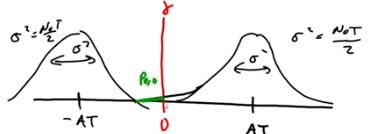
\includegraphics[scale=0.6]{Figures/Baseband_Binary/error_s0_transmitted_s1_detected}
\caption{Error Probability as Area under the curve: the tails of the Gaussian distribution}
\label{fig:Baseband_Binary:error_s0_transmitted_s1_detected}
\end{figure}

\end{itemize}

\end{frame}

\begin{frame}[t,allowframebreaks]{Computing $P \, (\text{Error} \, | \, s_2(t) \text{ is sent})$}

\begin{itemize}

\item Computing:

\begin{equation}
\begin{array}{rcl}
P \, (\text{Error} \, | \, s_2(t) \text{ is sent}) \, &=& \, P (V \, \leq \, \underbrace{k}_{ = \, 0} \, | \, s_2(t) \text{ is sent}) \\ \\
&=& \, P (V_2 \, \leq \, 0 \,)
\end{array}
\end{equation}



\item $P (V_2 \, \leq \, 0 \,)$ can be computed using the \textcolor{red}{cumulative distribution of the distribution}

\newpage
\item Cumulative distribution reminder for a Gaussian:

\begin{equation}
\begin{array}{rcl}
F(X \, = \, x) \, &=& \, P(X \, \leq \, x) \\ \\
				  &=& \, \Phi \left(\, \displaystyle\frac{x \, - \, E[X]}{ \sqrt{\text{Var}(X)} } \, \right)
\end{array}	
\end{equation}

	\begin{itemize}
	
	\item The random variable $X$ is the the conditional distribution $V_2$	
	
	\item $x \, = \, k$ the threshold value
	
	\item $E[X] \, = \, E[V_2] \, = \, \text{Amp} \, \times \, T_{\text{sym}}$
	
	\item $ \text{Var}(X) \, = \, \text{Var}(V_2) \, = \, \displaystyle\frac{N_0 \, T_{\text{sym}}}{2}$
	\end{itemize}

\newpage
\item Applying:

\begin{equation}
\begin{array}{rcl}
P (V_2 \, \leq \, 0 \,) \, &=& \, \Phi \left(\, \displaystyle\frac{\gamma  \, - \, E[V_2]}{ \sqrt{\text{Var}(V_2)}}  \, \right) \\ \\
&=& \, \Phi \left(\, \displaystyle\frac{0  \, - \, \text{Amp} \, \times \, T_{\text{sym}}}{\sqrt{0.5 \, \times \, N_0 \, T_{\text{sym}}} } \, \right) \\ \\
&=& \, \Phi \left(\, \displaystyle\frac{ \, - \, \text{Amp} \, \times \, T_{\text{sym}}}{\sqrt{0.5 \, \times \, N_0 \, T_{\text{sym}}} } \, \right) \\ \\
&=& \, 1 \, - \, \Phi \left(\, \displaystyle\frac{ \, + \, \text{Amp} \, \times \, T_{\text{sym}}}{\sqrt{0.5 \, \times \, N_0 \, T_{\text{sym}}} } \, \right) \\ \\
\end{array}
\end{equation}

\newpage

\begin{equation}
\begin{array}{rcl}
P (V_2 \, \leq \, 0 \,) \, &=& \,  1 \, - \, \Phi \left(\, \displaystyle\frac{ \, + \, \text{Amp} \, \times \, T_{\text{sym}}}{\sqrt{0.5 \, \times \, N_0 \, T_{\text{sym}}} } \, \right) \\ \\


&=& \, Q \left(\, \displaystyle\frac{ \, + \, \text{Amp} \, \times \, T_{\text{sym}}}{\sqrt{0.5 \, \times \, N_0 \, T_{\text{sym}}} } \, \right)
\end{array}
\end{equation}



\end{itemize}



\end{frame}


\begin{frame}[t,allowframebreaks]{Computing $P \, (\text{Error} \, | \, s_1(t) \text{ is sent})$}

\begin{itemize}
\item Now we compute the $\mathrm{2}^{\mathrm{nd}}$ type of error

\item Be aware that in the computation of $\mathrm{2}^{\mathrm{nd}}$ type error, we compute the  \textcolor{red}{probability above the threshold} $k$

\end{itemize}

\begin{equation*}
\begin{array}{rcl}
P \, (\text{Error} \, | \, s_1(t) \text{ is sent}) \, &=& \, P (V \, > \, \underbrace{k}_{ = \, 0} \, | \, s_1(t) \text{ is sent})  \\ \\ 
	&=&  \, P (V_1 \, >  \, 0 \,) \\ \\
	&=&  \, 1 \, - \, \underbrace{P (V_1 \, \leq \, 0 \,)}_{\text{Using CDF}} \\ \\
	&=&  \, 1 \, - \, \Phi \left(\, \displaystyle\frac{0  \, - \, (\, - \, \text{Amp} \, \times \, T_{\text{sym}})}{\sqrt{0.5 \, \times \, N_0 \, T_{\text{sym}}} } \, \right)
\end{array}
\end{equation*}

\newpage

\begin{equation*}
\begin{array}{rcl}
P \, (\text{Error} \, | \, s_1(t) \text{ is sent}) \, &=&  \, 1 \, - \, \Phi \left(\, \displaystyle\frac{+ \, \text{Amp} \, \times \, T_{\text{sym}}}{\sqrt{0.5 \, \times \, N_0 \, T_{\text{sym}}} } \, \right) \\ \\
&=&  \, Q \left(\, \displaystyle\frac{ \, + \, \text{Amp} \, \times \, T_{\text{sym}}}{\sqrt{0.5 \, \times \, N_0 \, T_{\text{sym}}} } \, \right)
\end{array}
\end{equation*}


\end{frame}

\begin{frame}[t]{Summary for Conditional Probabilities of Errors}

\begin{itemize}

\item $ P \, (\text{Error} \, | \, s_1(t) \text{ is sent}) \, = \, Q \left(\, \displaystyle\frac{ \, + \, \text{Amp} \, \times \, T_{\text{sym}}}{\sqrt{0.5 \, \times \, N_0 \, T_{\text{sym}}} } \, \right)$

\item  $P \, (\text{Error} \, | \, s_2(t) \text{ is sent}) \, = \, Q \left(\, \displaystyle\frac{ \, + \, \text{Amp} \, \times \, T_{\text{sym}}}{\sqrt{0.5 \, \times \, N_0 \, T_{\text{sym}}} } \, \right)$

\item What we have is that the \textcolor{red}{conditional probabilities} of \textcolor{red}{both error types} are the \textcolor{red}{same}:

	\begin{itemize}
	\item $P \, (\text{Error} \, | \, s_1(t) \text{ is sent}) \, = \, P \, (\text{Error} \, | \, s_2(t) \text{ is sent}) \, = \,  Q \left(\, \displaystyle\frac{ \, + \, \text{Amp} \, \times \, T_{\text{sym}}}{\sqrt{0.5 \, \times \, N_0 \, T_{\text{sym}}} } \, \right)$
	\end{itemize}

\end{itemize}

\end{frame}

\begin{frame}[t,allowframebreaks]{Total Probability of Error}

\begin{itemize}

\item We haven't done yet: don't forget that we are interested by the \textcolor{red}{total probability of the error}
\end{itemize}

\begin{equation*}
\begin{array}{rcl}
P(\text{Error}) \, &=& \, P \,( \,\text{Error} \, \cap \, s_1(t) \,) \, + \, P \, (\, \text{Error} \, \cap \, s_2(t) \, ) \\ \\
		 &=& \, P \,[\, s_1(t) \,] \, \times \, P \, (\, \text{Error} \, | \, s_1(t) \text{ is sent} \,)   \\
		&& + \,  P \, [ \,s_2(t) \, ] \, \times \,P \, \,(\, \text{Error} \, | \, s_2(t)\text{ is sent} \,) \\ \\
		&=& \, \displaystyle\frac{1}{2} \, Q \left(\, \displaystyle\frac{ \, + \, \text{Amp} \, \times \, T_{\text{sym}}}{\sqrt{0.5 \, \times \, N_0 \, T_{\text{sym}}} } \, \right) \, + \, \displaystyle\frac{1}{2} \, Q \left(\, \displaystyle\frac{ \, + \, \text{Amp} \, \times \, T_{\text{sym}}}{\sqrt{0.5 \, \times \, N_0 \, T_{\text{sym}}} } \, \right) \\ \\
		&=& \,Q \left(\, \displaystyle\frac{ \, + \, \text{Amp} \, \times \, T_{\text{sym}}}{\sqrt{0.5 \, \times \, N_0 \, T_{\text{sym}}} } \, \right) \, = \, Q \left(\, \displaystyle\frac{ \, + \, \sqrt{\text{Amp}^2 \, \times \, T^2_{\text{sym}}} }{\sqrt{0.5 \, \times \, N_0 \, T_{\text{sym}}} } \, \right)
\end{array}
\label{Eq:Baseband_Binary:proba_error_2}
\end{equation*}



\newpage 

\begin{equation*}
\begin{array}{rcl}
P(\text{Error}) \, &=& \,Q \left(\, \displaystyle\sqrt{\frac{ \, + \, 2 \, \text{Amp}^2 \, \times \, T_{\text{sym}} }{N_0}}  \, \right)
\end{array}
\label{Eq:Baseband_Binary:proba_error_3}
\end{equation*}

\begin{itemize}
\item Another observation we have: \textcolor{red}{total probability of error} is the \textcolor{red}{same} as the \textcolor{red}{conditional probability of errors}

	\begin{itemize}
	\item $P(\text{Error}) \, = \,  P \, (\text{Error} \, | \, s_1(t) \text{ is sent}) \, = \, P \, (\text{Error} \, | \, s_2(t) \text{ is sent}) \, = \, Q \left(\, \displaystyle\sqrt{\frac{ \, + \, 2 \, \text{Amp}^2 \, \times \, T_{\text{sym}} }{N_0}}  \, \right)$
	\end{itemize}
\end{itemize}

\end{frame}

\subsubsection{Probability of Error and SNR}


\begin{frame}[t,allowframebreaks]{Probability of Error and SNR}


\begin{itemize}

\item It is very common to use to express $P(\text{Error})$ as function of SNR

\item Computing the energy of the signals $s_i(t)$:

\end{itemize}

\begin{equation*}
\begin{array}{rcl}
\text{Energy} \, &=& \, \displaystyle\int\limits_{0}^{T_{\text{sym}}} [\, s_i(t) \,]^2 \, dt  \\ \\
		&=& \, \displaystyle\int\limits_{0}^{T_{\text{sym}}} [\, \text{Amp}  \,]^2 \, dt  \\ \\
		&=& \,\text{Amp} \, \times \, T_{\text{sym}}
\end{array}
\end{equation*}


\newpage
\begin{itemize}

\item Linking Formula of $P(\text{Error})$ and SNR using Energy expression:

\end{itemize}

\begin{equation*}
\begin{array}{rcl}
P(\text{Error}) \, &=& \, Q \left(\, \displaystyle\sqrt{\frac{ \, + \, 2 \, \text{Amp}^2 \, \times \, T_{\text{sym}} }{N_0}}  \, \right)  \\ \\
&=& \, Q \left(\, \displaystyle\sqrt{\frac{ \, + \, 2 \, \text{Energy} }{N_0}}  \, \right)  \\ \\
\end{array}
\end{equation*}

\newpage
\begin{itemize}

\item The quantity $ \displaystyle\frac{\text{Energy}}{N_0}$ is what we call \textcolor{red}{signal to noise ration} (SNR) and will commonly used in our analysis


\item SNR is often a big quantity, so we in practice we express it in dB
\end{itemize}

\begin{equation}
 \left( \,  \displaystyle\frac{\text{Energy}}{N_0}  \,\right)_{\text{dB}} \, = \, 10 \, \text{log}_{10} \,  \left( \,  \displaystyle\frac{\text{Energy}}{N_0}  \,\right)_{\text{Linear}}
\end{equation}

\begin{itemize}

\item Figure shows the $P(\text{Error})$ as function of SNR in dB

\begin{figure}[h]
\centering
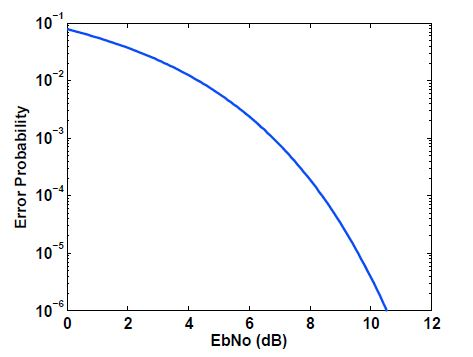
\includegraphics[scale=0.6]{Figures/Baseband_Binary/error_snr_dB}
\caption{$P(\text{Error})$ as function of SNR in dB scale}
\label{fig:Baseband_Binary:error_snr_dB}
\end{figure}

\end{itemize}

\end{frame}


\begin{frame}[t]{Common Mistake}

\begin{itemize}

\item When using the formula $ P(\text{Error}) \, = \, Q \left(\, \displaystyle\sqrt{\frac{ \, + \, 2 \, \text{Energy} }{N_0}}  \, \right)$ to know for example for a given energy of a signal, what is the probability of error, remember to \textcolor{red}{convert the SNR to linear before plug it int the equation of $P(\text{Error})$}

\end{itemize}

\end{frame}


\subsubsection{General Receiver}


\begin{frame}[t]{Generalization of Receiver Computation}

\begin{itemize}

\item Now we have understand the basic computation for receiver,
we will \textcolor{red}{generalize the concepts} done before

	\begin{itemize}
	\item However, we will \textcolor{red}{still in} the case of \textcolor{red}{binary digital communication} system 
	\end{itemize}

\item The receiver job was to do some kind of processing to give us a decision statistics which help us distinguish between the signals transmitted

\item  This decision statistics was compared to some threshold $k$

\item What we will generalize:

	\begin{itemize}
	\item Integration $\rightarrow$ filtering:
	
		\begin{itemize}
		\item Before the filtering operation was an integration operation, but is is the best one ?
		\end{itemize}

	\item $P(\text{error})$	
	
	\item Signals Shape:
	
		\begin{itemize}
		\item The transmitted signals $s_i(t)$ had a rectangular shape, what happen if we change the shape of these signals $\leftrightarrow$ try other forms then rectangular pulse ?
\end{itemize}			
	
	\end{itemize}


\end{itemize}

\end{frame}

\begin{frame}[t,allowframebreaks]{Generalization of Systems}


\begin{figure}[h]
\centering
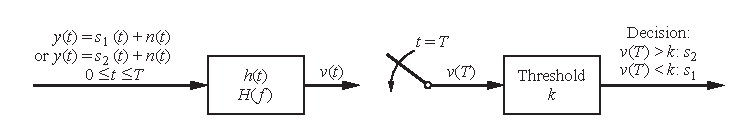
\includegraphics[scale=0.8]{Figures/Baseband_Binary/general_rx_binary}
\label{fig:Baseband_Binary:general_rx_binary}
\end{figure}


\begin{itemize}

\item We can see now that instead of $\displaystyle\int\limits_0^{T_{\text{sym}}}$ we have a \textcolor{red}{general linear system} $h(t)$

	\begin{itemize}
	\item The output of $h(t)$ is a random process $n(t)$
	
	\item It will be assumed to be Zero-Mean Wide-Sense Stationary Gaussian Random Process
	\end{itemize}

\item We sample a value from this random process at a time $T_0$

	\begin{itemize}
	
	\item So instead of $V$ we will have $V(T_0)$	
	
	\item Before, the time instant was $T_0 \, = \, T_{\text{sym}}$
	
	\item We determine later the \textcolor{red}{optimum sampling time}
	\end{itemize}


\newpage

\item As a receiver decision, we still have to compare $V(T_0)$ to some threshold $k$

\item Decision Rule:

	\begin{enumerate}
	\item $s_2(t)$ is sent if $V(T_0) \, > \, k$
	
	\item $s_1(t)$ is sent if $V(T_0) \, < \, k$ 
	\end{enumerate}

\item We could also reverse the above convention if we consider signal $s_2(t)$ is the one need to be in the left side and $s_1(t)$ in the right side

	\begin{enumerate}
	\item $s_1(t)$ is sent if $V(T_0) \, > \, k$
	
	\item $s_2(t)$ is sent if $V(T_0) \, < \, k$ 
	\end{enumerate}

\end{itemize}

\end{frame}

\begin{frame}[t]{Generalization of Signals}

\begin{itemize}

\item General transmitted signals $s_i(t)$ will be written as:

\begin{equation}
\begin{array}{rcl}
s_1(t) \, &=& \,\text{Amp} \, \times \, \psi_1(t) \\ \\
s_2(t) \, &=& \,\text{Amp} \, \times \, \psi_2(t)
\end{array}
\end{equation}

where $\psi_1(t)$ and $\psi_2(t)$ are \textcolor{red}{arbitrary shape signal} (rectangular, triangular, cos, $\cdots$) with \textcolor{red}{finite energy} signals on $[\, 0 \, , \,T_{\text{sym}} \,]$

\end{itemize}

\end{frame}


\begin{frame}[t,allowframebreaks]{Filter Output}

\begin{itemize}

\item The received signal $y_{R_x}(t)$:

\begin{equation}
y_{R_x}(t) \, = \, s_i(t) \, + \, n(t)
\end{equation}

\item $y_{R_x}(t)$ will be inputted to linear system $h(t)$, in which will give some output $V(t)$

\item We will apply superposition property to compute $V(t)$:

$$ s_i(t) \, \rightarrow \, h(t) \, \rightarrow s_{i_{\text{filtered}}}(t) $$

$$  n(t) \, \rightarrow \, h(t) \, \rightarrow \, n_{\text{filtered}}(t) $$

$$ y_{R_x}(t) \rightarrow \, h(t) \, \rightarrow V(t) $$

\begin{equation}
V(t) \, = \, \underbrace{s_{i_{\text{filtered}}}(t)}_{\text{deterministic}}  \, + \, \underbrace{n_{\text{filtered}}(t)}_{\text{probabilistic}}   
\end{equation}

\item The deterministic part of the filter output will give us the mean of $V(t) \, \leftrightarrow$ will tell us where to land on the real axis

	\begin{itemize}
	\item $s_{i_{\text{filtered}}}(t)$ can computed using convolution
	\end{itemize}

\begin{equation}
\begin{array}{rcl}
s_{i_{\text{filtered}}}(t) \, &=& \,  (\,s \, \star h \,)(t) \\ \\
&=& \, \displaystyle\int\limits_{- \, \infty}^{+ \infty} s_i(t \, - \, \tau) \, h(\tau) \, d\tau
\end{array}
\end{equation}

	\begin{itemize}
	\item $ s_i(t \, - \, \tau)$: we do a time reverse then shifting
	\end{itemize}

\newpage 

\item The challenging part as always is the probabilistic part $ n_{\text{filtered}}(t)$

\item However, we are assuming that $n(t)$ is a Gaussian random process with 0 mean

	\begin{itemize}
	\item If we filter a Gaussian process, we obtain a Gaussian process
	
	\item The mean of the output is 0 since we are assuming the input Gaussian process has 0 mean
	
	\item Need to \textcolor{red}{compute its variance}
	\end{itemize}
  
\item From random process theory, we can characterize the \textcolor{red}{variance} of the \textcolor{red}{output of a random process} from  \textcolor{red}{2 perspective}: 

	\begin{enumerate}
	\item Time using autorcorrolation
	
	\item Frequency using power spectral density
	\end{enumerate} 
 
 
\end{itemize}

\end{frame}


\begin{frame}[t,allowframebreaks]{Filter Output: Variance Computation using Time Domain}


\begin{itemize}

\item The autocorrolation $R_{n_{\text{filtered}}}(\tau)$:

\begin{equation}
\begin{array}{rcl}
R_{n_{\text{filtered}}}(\tau) \, &=& \, \displaystyle\int\limits_{- \, \infty}^{+ \, \infty} f (\tau \, - \, \lambda) \, R_{n_{\text{input}}} (\lambda) \, d\lambda
\end{array}
\label{Eq:baseband_binary_com:autorcorrolation_filtered_random_process}
\end{equation}

where 

\begin{equation}
f(t) \, = \, \displaystyle\int\limits_{- \, \infty}^{+ \, \infty} h (u \, - \, t) \, h(u) \, du
\label{Eq:baseband_binary_com:autorcorrolation_filtered_random_process_2}
\end{equation}


\item Equation (\autoref{Eq:baseband_binary_com:autorcorrolation_filtered_random_process}) are general equation for any input random process $n_{\text{input}}(t)$

	\begin{itemize}
	\item However, in our case $n_{\text{input}}(t)$ is a Gaussain white noise so its autocorrolation is $N_0 \, \delta(\lambda)$
	\end{itemize}

\item Developing equation (\autoref{Eq:baseband_binary_com:autorcorrolation_filtered_random_process}) we have:

\begin{equation}
\begin{array}{rcl}
R_{n_{\text{filtered}}}(\tau) \, &=& \, \displaystyle\int\limits_{- \, \infty}^{+ \, \infty} f (\tau \, - \, \lambda) \, R_{n_{\text{input}}} (\lambda) \, d\lambda \\ \\
	&=& \, \displaystyle\int\limits_{- \, \infty}^{+ \, \infty} f (\tau \, - \, \lambda) \, 0.5 \,  N_0 \, \delta(\lambda) \, d\lambda
\end{array}
\end{equation}

\newpage

\begin{equation}
\begin{array}{rcl}
R_{n_{\text{filtered}}}(\tau) \, &=& \, 0.5 \,  N_0 \, \displaystyle\int\limits_{- \, \infty}^{+ \, \infty} f (\tau \, - \, \lambda)  \, \delta(\lambda) \, d\lambda \\  \\
 &=& \, 0.5 \,  N_0 \, f (\tau)\, \displaystyle\int\limits_{- \, \infty}^{+ \, \infty}  \delta(\lambda) \, d\lambda \\  \\
 &=& \, 0.5 \,  N_0 \, f (\tau)\, \times \, 1 \\ \\
 &=& \, 0.5 \,  N_0 \, f (\tau)
\end{array}
\end{equation}

And $\text{Var}(n_{\text{filtered}}) \, = \, R_{n_{\text{filtered}}}(\tau \, = \, 0)$

\end{itemize}

\end{frame}

\begin{frame}[t]{Filter Output: Variance Computation using Frequency Domain}

\begin{itemize}

\item Using power spectral density we have:

\begin{equation}
S_{n_{\text{filtered}}}(\omega_c) \, = \, |H(\omega_c)| \, \times \, S_{n_{\text{input}}}(\omega_c)
\end{equation}

\item For a white noise $S_{n_{\text{input}}}(\omega_c) \, = \, 0.5 \, N_0$

\end{itemize}

\end{frame}

\begin{frame}[t]{Decision Statistics $V$}

\begin{itemize}

\item Once we analyze the filter output, the next step is to grad a sample at some time instant $T_0$

\item The decision statistic $V(T_0)$ which is the \textcolor{red}{input to the threshold device} is written as:

\begin{equation}
V(T_0) \, = \, s_{i_{\text{filtered}}}(t \, = \, T_0) \, + \, n_{\text{filtered}}(t \, = \, T_0)
\end{equation}

\item Assuming signal $s_2(t)$ is transmitted, we can write (same as we did in before) \textcolor{red}{conditioned decision statistic} $V_2(T_0)$

\begin{equation}
\begin{array}{rcl}
V_2(T_0) \, &=& \, V(T_0 \, | \, s_2(t) \text{ is transmitted}) \\ \\
 &=& \, s_{2_{\text{filtered}}}(t \, = \, T_0) \, + \, n_{\text{filtered}}(t \, = \, T_0)
\end{array}
\end{equation}

\item We will \textcolor{red}{compute} its mean $ E[\,V_2(T_0)  \,]$ and its variance $\text{Var} ( \, V_2(T_0)  \, )$ as \textcolor{red}{function of the grabbing time} $T_0$ so we can \textcolor{red}{optimize upon $T_0$} later

\end{itemize}

\end{frame}

\begin{frame}[t,allowframebreaks]{Expectation of Decision Statistics $V_2$}

\begin{equation*}
\begin{array}{rcl}
E[\,V_2(T_0)  \,] \, &=& \, E \left[\,  s_{2_{\text{filtered}}}(t \, = \, T_0) \, + \, n_{\text{filtered}}(t \, = \, T_0)    \,\right] \\ \\
 &=& \, E \left[ \, \underbrace{s_{2_{\text{filtered}}}(t \, = \, T_0)}_{\text{deterministic}}  \,  \right] + \, E \left[ \, n_{\text{filtered}}(t \, = \, T_0)    \, \right] \\ \\
  &=& \, s_{2_{\text{filtered}}}(t \, = \, T_0) \, + \, 0 \\ \\
  &=& \,  \displaystyle\int\limits_{- \, \infty}^{+ \infty} s_2(T_0 \, - \, \tau) \, h(\tau) \, d\tau
\end{array}
\end{equation*}

\newpage
\begin{itemize}

\item As summary we have:

\begin{equation}
E[\,V_2(T_0)  \,] \, = \, \displaystyle\int\limits_{- \, \infty}^{+ \infty} s_2(T_0 \, - \, \tau) \, h(\tau) \, d\tau
\label{Eq:baseband_binary_com:mean_conditional_decision_statistic}
\end{equation}

Equation (\autoref{Eq:baseband_binary_com:mean_conditional_decision_statistic}) is a generic equation:

	\begin{itemize}
	\item We have a general system $h$

	\item A general sampling time $T_0$ to choose from
	
	\item A general shape of the transmitted signal $s_2(t)$
	\end{itemize}

\end{itemize}

\end{frame}

\begin{frame}[t,allowframebreaks]{Variance of Decision Statistics $V_2$}

\begin{equation*}
\begin{array}{rcl}
\text{Var}[\,V_2(T_0)  \,] \, &=& \, E \left[\, (\, V_2(T_0) \, - \,  E[\,V_2(T_0)  \,]  \,)^2 \,\right] \\ \\
 &=& \, E [\, (\, s_{2_{\text{filtered}}}(t \, = \, T_0) \, + \, n_{\text{filtered}}(t \, = \, T_0) \, - \, \\ 
 && s_{2_{\text{filtered}}}(t \, = \, T_0)\,]  \,)^2 \,] \\ \\
  &=& \,   E \left[\, (\, n_{\text{filtered}}(t \, = \, T_0) \,)^2 \,\right] 
\end{array}
\end{equation*}

\begin{itemize}
\item  As always, the variance is a function of the noise $n_{\text{filtered}}(t \, = \, T_0)$, and has nothing to do with the transmitted signals $s_2(t)$

\item Now the expression $ E \left[\, (\, n_{\text{filtered}}(t \, = \, T_0) \,)^2 \,\right]$ is of the form $E[X^2]$ for a random variable $X$

\item We can do also the same steps when we did the computation for $\text{Var}(V_2)$ in the integration-and-dump rx and decompose the integral to an multiplication of integrals  $\leftrightarrow \, \displaystyle\int \, \times \,\displaystyle\int$

	\begin{itemize}
	\item But we will skip the computation for now
	\item To be done later
	\end{itemize}

\item As summary we have as final answer:

\begin{equation}
\text{Var}[\,V_2(T_0)  \,] \, = \,R_{n_{\text{filtered}}} (\tau \, = \, 0)
\end{equation}

\end{itemize}



\end{frame}


\begin{frame}[t]{Conditional Distribution Plots}

\begin{figure}[h]
\centering
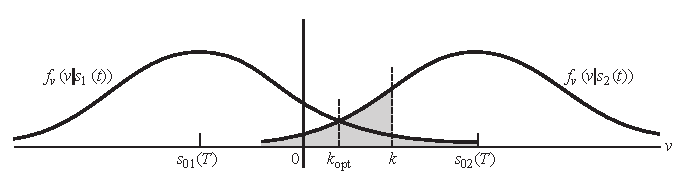
\includegraphics[scale=0.8]{Figures/Baseband_Binary/conditional_distribution_plots}
\caption{Conditional probability density functions of the filter output at time $t \, T_0$}
\label{fig:Baseband_Binary:conditional_distribution_plots}
\end{figure}

\begin{itemize}

\item Since we have 2 signals to choose from, 1 threshold line is enough to decide which signal I have

\end{itemize}

\end{frame}

\begin{frame}[t]{Probability of Error}

\begin{itemize}

\item Once I have decided my threshold line where, the next step is to compute the $P(\text{Error})$

	\begin{itemize}
	\item For now, we skip the problem of finding the optimum value for the threshold $k$
	
	\item We do it in next sections
	\end{itemize}
	 

\end{itemize}

\end{frame}


%------------ References ------------------------
\section{References}


\begin{frame}[allowframebreaks]
\frametitle{References}

\bibliographystyle{IEEEtran}
\frametitle{References}
\bibliography{literature/Communication_Systems}

\end{frame}


\end{document}

